%%%%%%%%%%%%%%%%%%%%%%%%%%%%%%%%%%%%%%%%%
% written by: Ruben (rg@ht11.org)
%%%%%%%%%%%%%%%%%%%%%%%%%%%%%%%%%%%%%%%%%

\documentclass{article}
\usepackage{fancyhdr} % Nice headers
\usepackage{lastpage} % Required to determine the last page for the footer
\usepackage{extramarks} % Required for headers and footers
\usepackage{graphicx} % Required to insert images
\usepackage{listings} % Required for insertion of code
\usepackage{courier} % Required for the courier font
\usepackage[hidelinks]{hyperref} % I hate hyperlinks in docs...
\usepackage[utf8]{inputenc} % because äöü
\usepackage{setspace} % Spacing between rows

% Margins
\topmargin=-0.45in
\evensidemargin=0in
\oddsidemargin=0in
\textwidth=6.5in
\textheight=9.0in
\headsep=0.25in

\linespread{1.1} % Line spacing

% Set up the header and footer
\pagestyle{fancy}
% \lhead{Ruben Gonzalez} % Top left header
\chead{Computer Networks Cheat Sheet} % Top center head
\rhead{} % Top right header
\lfoot{\copyright Ruben, released under the BEERWARE license} % Bottom left footer
\cfoot{} % Bottom center footer
\rfoot{Page\ \thepage\ of \pageref*{LastPage}} % Bottom right footer, * so hyperref doesnt link it.
\renewcommand\headrulewidth{0.4pt} % Size of the header rule
\renewcommand\footrulewidth{0.4pt} % Size of the footer rule

\setlength\parindent{0pt} % Removes all indentation from paragraphs

\begin{document}
\section{Packet Delay}
\subsection{Definitions}
\textbf{Link capacity}
Capacity of link. Unit: $\frac{Bits}{Seconds}$.

\textbf{Transmission Delay}
Time needed to bring bytes of packet onto link. Calculated: $d_{trans} = \frac{B}{R}$, with B = bits per packet and R = Link Capacity.

\textbf{Propragation Delay}
Time neeeded to transmit one bit from one end of the link to the other. 

\textbf{Processing Delay}
Time needed to proccess packet.

\textbf{Queueing Delay}
Time spend waiting in buffer queues.

\textbf{Overall Delay}
Calculated: $d_{nodal} = d_{proc} + d_{queue} + d_{trans} + d_{prop}$

\textbf{End to End Delay}
Also Known as one way delay. Time needed for packet to go from sender to receipient. Usually $\frac{RTT}{2}$. Excact: $\sum\limits_{i}^{n} d_{i}$, with $d_{i}$ = overall delay of network segment i.

\section{HTTP}
\subsection{Definitions}
\textbf{Non Persistent HTTP}
One HTTP request per TCP connection.

\textbf{Persistent HTTP}
Multiple HTTP request per TCP connection. Still one request at a time, next HTTP request gets send after previous HTTP request is done.

\textbf{Pipelining HTTP}
Introduced in HTTP/1.1. Send multiple ordered requests simultaniously, without waiting for previous requests to be done.

\begin{figure}[h]
    \centering
    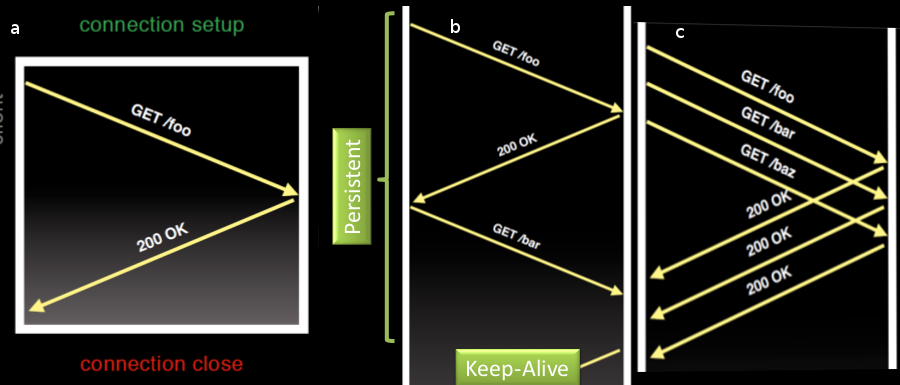
\includegraphics[width=0.9\textwidth]{media/http.png}
    \caption{Different HTTP versions. a non persistent, b persistent, c pipelined HTTP}
    \label{fig:pipe_http}
\end{figure}

\pagebreak

\section{TCP Flow Control}
\subsection{Definitions}
\label{sbsec:flow_defs}
\textbf{Window}
Bytes allowed to be sent before receiving next ACK.


\textbf{Window Size}
Size of window. Basically size of receipient buffer.

\textbf{Advertised Window}
Receipients Window Size told to sender of TCP packets. Maximum size allowed for window.

\textbf{Maximum Segment Size (MSS)}
Payload size in bytes. Usually MTU - len(IP header) - len(TCP header), on ethernet MSS=1460.

\textbf{Window}
Bytes allowed to be sent before receiving next ACK.

\textbf{Segment}
TCP packet. Consists of header and data.

\textbf{Sequence Number (SEQ)[header field]}
Numbering of data within segment. SEQ = first byte in the payload (data) of segment. Gets initialized to random number (ISN) at start of connection.

\textbf{Acknowledge Number (ACK)[header field]}
Acknowledgement of received segments. Value is SEQ + 1, with SEQ = segment number of received segment.

\subsection{Sliding Window}
Every time a ACK returns, the sender slides the Window over the bytes to send.
\begin{figure}[h]
    \centering
    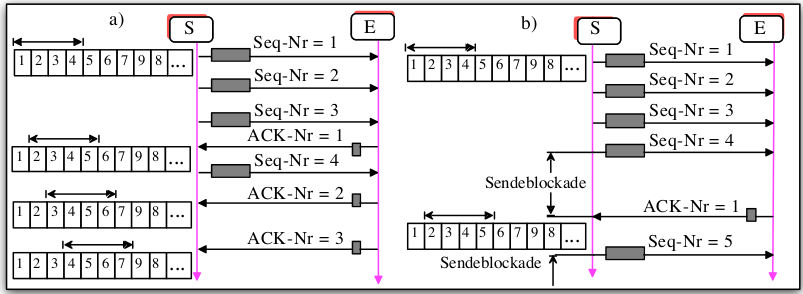
\includegraphics[width=0.6\textwidth]{media/sliding_window.png}
    \caption{Sliding window with Window Size = 4, a without, b with error}
    \label{fig:sliding}
\end{figure}


\section{TCP Efficency Tuning}
\subsection{Definitions}

\textbf{Congestion Window (cwnd)}
The same as Window, see \ref{sbsec:flow_defs}.

\textbf{Slow Start Threshhold (ssthresh)}
Limit until exponential growth (Slow Start) of cwnd is performed. After $cwnd \geq sstresh$, linear growth (congestion avoidance) is performed.

\textbf{Double ACK (dACK)}
In case a segment is missing, the ACK for the already arrived segment with bigger SEQ is repeadiately sent.

\textbf{Packet loss}
Paket is considered lost if either the timeout for ACK is reached, or 3 dACKs have arrived.

\subsection{Slow Start}
Algorithm to perform exponential growth of cwnd.

Begins with $cwnd = 1 \cdot MSS$ and performs $cwnd = cwnd + MSS$ on every received ACK.

\subsection{Congestion Avoidance}
Algorithm to perform linear growth of cwnd if needed.

In case $cwnd \geq sstresh$ occures, cwnd gets increased $cwnd = cwnd + \frac{MSS^{2}}{cwnd}$ everytime a ACK arrives. Otherwise Slow Start is performed.

Congestion avoidance begins with these steps:

\begin{enumerate}
     \item Set $ssthresh = 2^{16} -1 = 65535$
     \item Begin with slow start.
\end{enumerate}

In case a packet loss gets detected, the following is done:

\begin{itemize}
     \item In case a timeout occured: set $ssthresh = max(2, \frac{cwnd}{2})$ and do slow start
     \item In case 3 dACKs were received: only set $ssthresh = max(2, \frac{cwnd}{2})$ (as in 1.)
\end{itemize}

\subsection{Fast Retransmit}
Mechanism that means: On third dACK received, the missing segment gets resent immediately without waiting for timer to expire.

\subsection{Fast Recovery}
Mechanism that means: After fast retransmit, congestion avoidance is performed not slow start.

The usual implementation looks like this: If third dACK is received do the following:

\begin{enumerate}
     \item Set $ssthresh = max(2, \frac{cwnd}{2})$
     \item Retransmit the missing segment
     \item Set $cwnd = ssthresh + 3 \cdot MSS$
     \item Every time another dACK arrives set $cwnd = cwnd + MSS$
     \item Once a ACK for new data arrives, set $cwnd = sstresh$.
\end{enumerate}

\subsection{Throughput}
\subsection{Definitions}

\textbf{Round Trip Time (RTT)}
Estimation of time needed from sending a package until receving an answer (after leaving link to the answer arriving).

\subsection{Bandwitdh Delay Product}
Measures the throughput: $bdp [\frac{byte}{sec}] = \frac{Windowsize [byte]}{RTT [sec]}$

\section{IP}
\subsection{Whats new}
The usual stuff. Use the most specific (smallest) subnet matching in routing.

\section{Routing Protocols}
\subsection{Routing Information Protocol}
Metric is the amount of Hops.

\subsection{Open Shortest Path First}
Metric for route: $\sum{\frac{100 Mbits}{Bandwidth}}$ of all links.

\subsection{Enhanced Gateway Routing Protocol}
Metric for route: $ \frac{10 Gbps}{min(Bandwidth)} + \sum\limits_{link i}^{n} \frac{D_i}{10\mu s}$, with D=Delay

\end{document}

